\documentclass[12pt,a4paper,utf8]{ctexart}
\usepackage{ctex,amsmath,amssymb,subfig,cite,graphicx,diagbox,fontspec,fancyhdr,geometry}
\usepackage[ntheorem]{empheq}
\usepackage{enumitem,fullpage,cleveref,cellspace,listings,color,framed}
\definecolor{gray}{rgb}{0.5,0.5,0.5}
\definecolor{dkgreen}{rgb}{.068,.578,.068}
\definecolor{dkpurple}{rgb}{.320,.064,.680}

%set Fortran styles
\lstset{
    frameround=tftf,
    language=Fortran,
    keywords={SELECT,PROGRAM,PRINT,STOP,END,WRITE,INTEGER,REAL,COMPLEX,CHARACTER,LOGICAL,READ,FORMAT,IMPLICIT,PARAMETER,DATA,EQUIVALENCE,TYPE,PAUSE,CONTINUE,CYCLE,EXIT,IF,SELECT,DO,ALLOCATE,DEALLOCATE,WHERE,FORALL,SUBROUTIHNE,CALL,RETURN,FUNCTION,COMMON,BLOCK DATA,SAVE,INTERFACE,CONTAIN,MODULE,USE,PUBLIC,PRIVATE,ENTRY,OPEN,INQUIRE,CLOSE,NAMELIST,POINTER,NULLFY,REWIND,BACKSPACE,ENDFILE
    },
    basicstyle=\small\ttfamily,
    numbers=left,
    numberstyle=\small,
    keywordstyle=\color{blue}\bfseries,
    commentstyle=\color{dkgreen},
    stringstyle=\color{dkpurple},
    backgroundcolor=\color{white},
    tabsize=2,
    showspaces=false,
    showstringspaces=false,
    breaklines=true,
    frame=trBL,
}
\CTEXsetup[format+={\raggedright}]{section}
\setlength{\parindent}{2em}
\geometry{
    textwidth=138mm,
    textheight=215mm,
    left=27mm,
    right=27mm,
    top=25.4mm,
    bottom=25.4mm,
    headheight=2.17cm,
    headsep=4mm,
    footskip=12mm,
    heightrounded,
}
\pagestyle{fancy}
\lhead{\textsl{2021秋-计算物理A}}
\chead{}
\rhead{\textsl{PB19020634-于浩然}}
\lfoot{}
\cfoot{\thepage}
\rfoot{}

\begin{document}
\begin{center}
    {\LARGE\textbf{计算物理作业十二}}\\
    \textrm{于浩然}~~~~~~\textrm{PB19020634}~~~~~~\textrm{2021.11.30}
\end{center}

\section{作业题目}

推导正方格子点阵上键逾渗的重整化群变换表达式$p' = R(p)$,求临界点$p_c$与
临界指数$\nu$,与正确值(表1.6.1.3-1)相比较.
\section{方法简介}
\subsection{逾渗阈值}

\textbf{逾渗}(percolation)是一种用于描述流体在无序介质中作随机扩展和流动的模型,
可以用来阐明相变和临界现象的一些重要物理概念. 

我们研究逾渗采用最基础的形式:在呈现某种几何构型的点阵上进行逾渗. 一个点阵由点
(键之间的交点)和键(点之间的连线)组成,点阵上的逾渗过程有两种类型:座(site)逾渗和
键(bond)逾渗. 
在这里我们仅说明键逾渗:每条键是连通的或非连通的,连通的概率为$p$,非连通的概率
为$1-p$. 

当$p=0$时,没有通路连通;随着$p$增大,总会达到一个临界浓度$p_c$,当$p > p_c$时总
存在跨越集团(从顶到底或从左到右),$p_c$即为所谓逾渗阈值. 

\subsection{临界指数}

首先定义集团的平均跨越长度$\xi$. 采用最简单的方法,将集团中的两条键的中心的最大
间距取作$\xi$,即
\begin{equation}
    \xi = \langle \max \{ | \mathbf{r}_i - \mathbf{r}_j|\}_{(i,j) \in cluster} \rangle 
\end{equation}

对于跨越长度$\xi(p)$,当$p < p_c$时,它是$p$的增函数;当$p > p_c$时,它趋于
系统的尺度$\infty$(对于排除了无穷大集团的定义式,当$p > p_c$时,它是$p$的减函数)
,因此用幂指数$\nu$来刻画$\xi$在临界区域的发散性:
\begin{equation}
    \xi(p)\sim |p-p_c|^{-\nu}
\end{equation}

我们真正关心的是$p < p_c$时的指数.
\subsection{实空间重整化群}

实空间重整化群是一种忽略细节从而减少自由度、简化物理问题的方法.
将点阵分为一个个尺度放大因子为$b$的元胞,考虑单个元胞能够连通的几率为$p'$
,则有重整化群变换表达式:
\begin{equation}
    p' = R(p,b)
\end{equation}

一般来说,重整化后的点阵占据几率$p'$与原格子点阵占据几率$p$不同.
经过不断地变换,结果要么趋向于完全不占据的不动点$p=0$,要么趋向于完全占据的
不动点$p=1$. 除去上面两个平凡的不动点之外,存在一个非平凡的不动点即$p^{\star} =
p_c$, 它应满足方程
\begin{equation}
    p^{\star} = R(p^{\star})
\end{equation}

为了计算临界指数,考虑重整化格子点阵中所有长度量应比原来缩小$b$倍,以保证系统在
标度变换下不变,即关联长度$\xi' = \xi / b$. 由上一小节中(2)式,有
\begin{equation}
    |p'-p^{\star}|^{-\nu} = b^{-1} |p-p^{\star}|^{-\nu}
\end{equation}
取一阶近似
\begin{equation}    
    p' - p^{\star} = \frac{ \textrm{d}R(p^{\star})}{ \textrm{d}p}
\end{equation}
上式两端取$\nu$次幂
\begin{equation}
    |p' - p^{\star}|^{\nu} = \left | \frac{ \textrm{d}R(p^{\star})}{
    \textrm{d}p} \right | ^{\nu}
\end{equation}

与(5)式比较,取对数可得
\begin{equation}
    \nu = \frac{\ln b}{\ln  \frac{ \textrm{d}R(p^{\star})}{ \textrm{d}p}}
\end{equation}

即所求临界指数. 

\section{推导过程}

首先推导正方格子上键逾渗的重整化群变换表达式. 

由于研究逾渗时
关心的是临界点附近从点阵的一侧到另一侧存在连接的通路,只需考虑单个元胞能否实现从一端到另
一端的连通. 与座逾渗所考虑的正方形元胞不同,研究键逾渗时我们考虑“工”形的元胞.
每个元胞形成一个方向为从左到右的“巨键(super
bonds)”,每个“巨键”只有连通和不连通两种状态,展示如下图. 
\begin{figure}[!h]
    \centering
    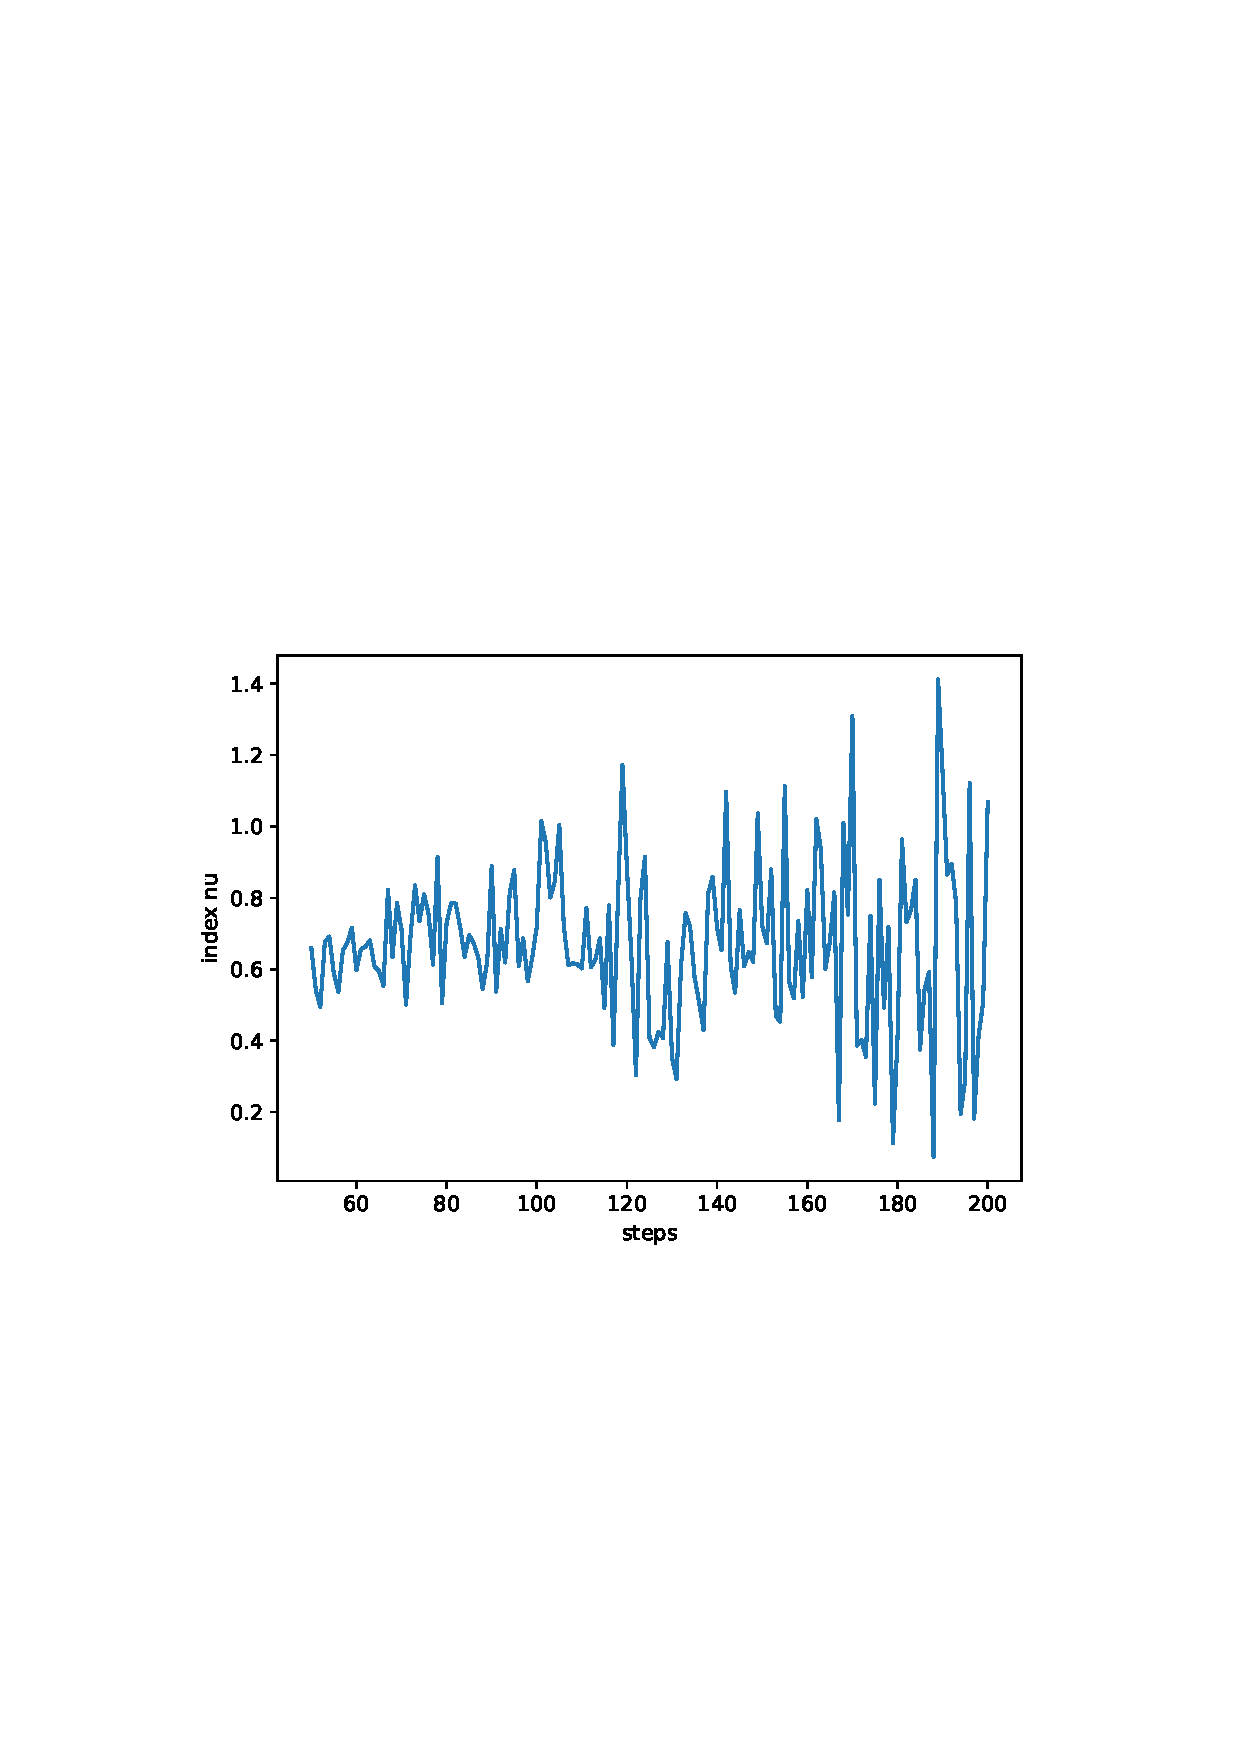
\includegraphics[width=0.4\textwidth]{fig1.png}
    \caption{“工”形元胞重整化为一个“巨键”}
\end{figure}

\newpage
考虑所有能够使元胞从左到右连通的情形,以及其概率如图二(上式中考虑了同一种元胞形式的
各种对称形式,体现为系数). 
\begin{figure}[!t]
    \centering
    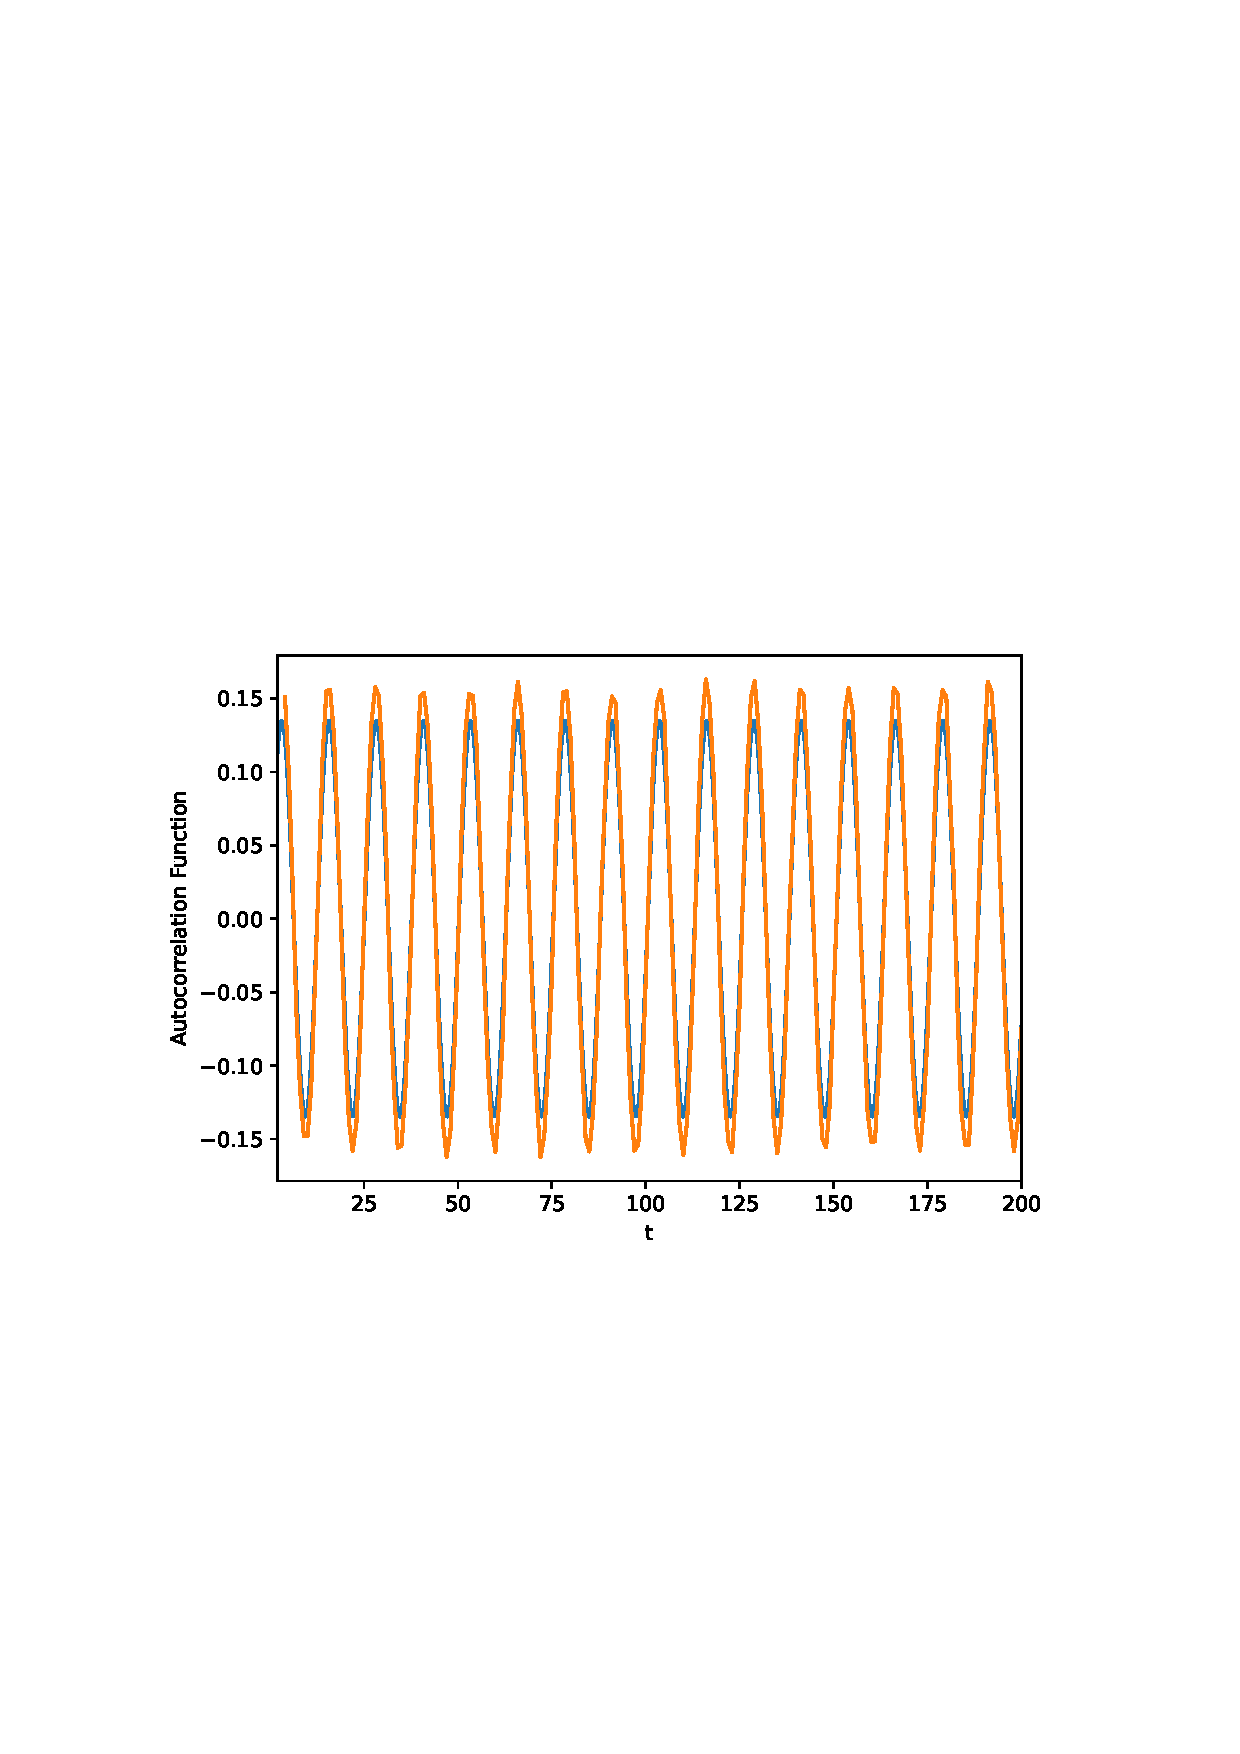
\includegraphics[width=0.8\textwidth]{fig2.png}
    \caption{元胞左右连通的情形与相应概率}
\end{figure}
重整化群变换即为一个“巨键”连通的概率,亦即上面的概率相加,得
\begin{eqnarray}
    p' &=& R(p) \nonumber \\
       &=& p^5 + P^4(1-p) + 4p^4(1-p) + 2p^3(1-p)^2 + 2p^3(1-p)^2 + 
       4p^3(1-p)^2 + 2p^2(1-p)^3 \nonumber \\
       &=& 2p^5 - 5p^4 + 2p^3 +2p^2
\end{eqnarray}
临界点$p^{\star}$满足不动点方程
\begin{equation}
    R(p^{\star}) = 2p^{\star 5}- 5p^{\star 4} + 2p^{\star 3} + 2p^{\star 2} =
    p^{\star}
\end{equation}
有三个解
\begin{equation}
    p^{\star}=
    \begin{cases}
        0\\ 1\\ 0.5
    \end{cases}
\end{equation}
$p^{\star}=0,1$均为平凡解,非平凡的不动点$p^{\star}=0.5$即为临界点$p_c$. 

对(9)式求导:
\begin{equation}
    \frac{ \textrm{d}p'}{ \textrm{d}p} = 10p^4 - 20p^3 + 6p^2 + 4p
\end{equation}

由图1所示重整化群机制易得尺度放大因子$b=2$,由(8)式可得临界指数:
\begin{equation}
    \nu = \frac{ \ln 2}{\ln \left . \frac{ \textrm{d}p'}{
        \textrm{d}p}\right|_{p=0.5}} = \frac{\ln 2}{\ln \frac{13}{8}} \approx 1.4277
\end{equation}

\section{结果分析与结论}

查阅表1.6.1.3-1可得,正方格子点阵上键逾渗的标准值为$p_c = 0.5,\nu = 4/3 \approx 1.6667$. 
可见,推导的临界点与标准值完全符合,临界指数有一定偏差但已经达到了较好的精度. 

通过做本次作业,对于研究逾渗和实空间重整化群的方法有了一定的认识.
\end{document}
